% The user manual. Build from this directory: latexmk -lualatex beamer-floral.tex
\documentclass[a4paper,11pt]{article}
\usepackage{fontspec}
\usepackage[margin=30mm]{geometry}
\usepackage{graphicx,booktabs,xcolor}
\usepackage{listings}
\usepackage{hyperref}
\hypersetup{colorlinks,linkcolor=black,urlcolor=blue!50!black,
  pdftitle={beamer-floral manual},pdfauthor={Kristian Niemi}}
\lstset{basicstyle=\ttfamily\small,columns=fullflexible,keepspaces,
  frame=single,framerule=.3pt,rulecolor=\color{black!30},
  upquote=true,breaklines=true}
\setlength\parindent{0pt}
\setlength\parskip{.6em}
\newcommand\pkg[1]{\textsf{#1}}
\newcommand\cmd[1]{\texttt{\textbackslash #1}}
\title{The \pkg{beamer-floral} package\\[.3em]\large Version 0.1.0}
\author{Kristian Niemi}
\date{8 November 2026}

\begin{document}
\maketitle

\pkg{beamer-floral} draws procedural watercolour flora behind \pkg{beamer}
slides. The drawing comes from \pkg{tikz-flora}. Each frame gets its own
plant; the package measures the text block, so the stems grow around the
content.

\begin{center}
  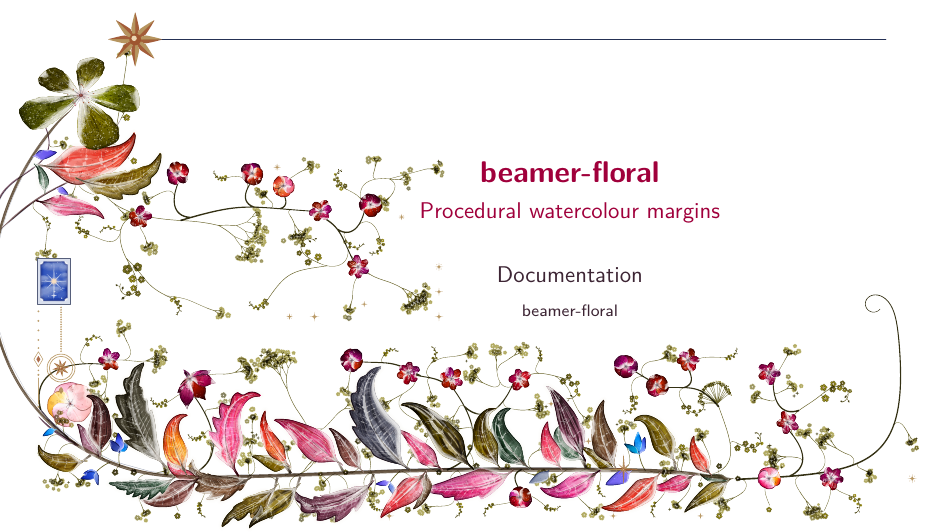
\includegraphics[width=.72\linewidth]{img/title.png}
\end{center}

\tableofcontents

\section{Requirements}

The package needs LuaLaTeX, \pkg{beamer} and \pkg{tikz-flora}. It has been
tested with TeX Live 2025.

\pkg{tikz-flora} is not distributed through CTAN. The integration needs
revision \texttt{39cfd26} or later of the branch \texttt{beamer-floral} at
\url{https://github.com/krissen/tikz-flora}. The release archive of
\pkg{beamer-floral} on GitHub includes a matching engine. To use a separate
checkout, set the environment variable \texttt{TIKZFLORA} to its path.

Timed growth also needs the \pkg{animate} package. Raster playback needs
Python 3.9 or later and Poppler's \texttt{pdftocairo} when its cache is
built.

\section{Getting started}

\begin{lstlisting}[language={[LaTeX]TeX}]
\documentclass{beamer}
\usetheme{floral}
\florasetup{seed=3, density=1.2}
\begin{document}
\begin{frame}{Floral}
  The border grows around the text.
\end{frame}
\end{document}
\end{lstlisting}

Compile with \texttt{latexmk -lualatex}. The package stores measurements in a
\texttt{.floral-cache} file and asks for a rerun when they change.

To keep a stock theme, load it first:

\begin{lstlisting}[language={[LaTeX]TeX}]
\usetheme{Madrid}
\usepackage{beamer-floral}
\end{lstlisting}

The package sets margins of 2.5\,cm on the left and 1\,cm on the right. Call
\cmd{setbeamersize} after loading it to change them.

\section{Commands}

\begin{description}
  \item[\cmd{florasetup}\{\emph{keys}\}] Sets the document's options.
  \item[\cmd{florathisframe}\{\emph{keys}\}] Sets options for the next
    painted frame, including all its overlays. \cmd{florathispage} is an alias.
  \item[\cmd{floraon}, \cmd{floraoff}] Switch the flora on or off before a frame.
  \item[\cmd{florapalette}\{\emph{name}\}] Selects \texttt{warm},
    \texttt{blue}, \texttt{green} or \texttt{green-stems}. With the floral
    theme it also sets block, alert and example colours.
  \item[\cmd{florareserve}\{\emph{x}\}\{\emph{y}\}\{\emph{x$_1$}\}\{\emph{y$_1$}\}]
    Keeps flora out of a rectangle. Arguments are dimensions from the
    lower-left corner of the page.
  \item[\cmd{floraclearreserve}] Removes all reservations.
  \item[\cmd{florabackground}{[}\emph{position}{]}\{\emph{colour}\}\{\emph{height}\}]
    Paints a band at the \texttt{top} or \texttt{bottom}. Height \texttt{0pt}
    removes it.
\end{description}

The floral theme adds \cmd{floralornamentsetup}, \cmd{floraldivider} and the
\texttt{floral} templates for \texttt{itemize item}, \texttt{itemize subitem}
and \texttt{itemize subsubitem}, and an optional section page,
\verb|\setbeamertemplate{section page}[floral]|: the section name beside the
flora with a divider below it, on a lighter version of the title page's
composition. It is not selected by default, and the theme adds no
\cmd{AtBeginSection} hook; the README shows the one-line hook. Every frame of the theme carries a
running-head mark at the top of the left margin; on a titled frame it sits
above the title, in a size that follows the room there.
\verb|tune={gesture={mark_min=10}}| sets the smallest mark drawn (10\,pt by
default); with less room the mark is left out. The mark is drawn whole or not
at all: no kind reaches above or below its square, and beside a reservation
the mark takes the largest whole size that fits, lower down or smaller, or is
left out; its rule stops short of the reservation. Pattern pages carry no mark.

\section{Options}

\begin{center}
\begin{tabular}{@{}lp{.68\linewidth}@{}}
  \toprule
  Key & Values \\
  \midrule
  \texttt{layout} & \texttt{left}, \texttt{right}, \texttt{centered},
    \texttt{split}, \texttt{title}, \texttt{surround} \\
  \texttt{header} & \texttt{body}, \texttt{margin} \\
  \texttt{seed} & a number, or \texttt{random} \\
  \texttt{density} & 0 to 10 \\
  \texttt{mix} & weights such as \texttt{\{leaves=3, leaflets=2\}} \\
  \texttt{visitors} & weight for bees, butterflies, birds and snails \\
  \texttt{colourway} & \texttt{spring}, \texttt{summer}, \texttt{autumn},
    \texttt{winter}, \texttt{ember}, \texttt{plum}, \texttt{rose},
    \texttt{original} \\
  \texttt{palette} & inks such as \texttt{\{hero=gold, blooms=blue\}} \\
  \texttt{spin} & re-picks random inks \\
  \texttt{ornaments} & weights of registered ornament kinds \\
  \texttt{tune} & engine overrides \\
  \texttt{growth} & \texttt{off}, \texttt{overlays}, \texttt{timed} \\
  \texttt{growth duration} & seconds, default 8 \\
  \texttt{growth fps} & an integer from 1 to 60, default 20 \\
  \texttt{reuse} & \texttt{none}, \texttt{all}, or a list of \texttt{title},
    \texttt{section}, \texttt{content} \\
  \texttt{stage} & \texttt{off} (default), \texttt{right}, \texttt{left} \\
  \texttt{stage width} & a length, default \texttt{0.39\textbackslash paperwidth} \\
  \texttt{stage margin} & a length, default \texttt{12mm} \\
  \bottomrule
\end{tabular}
\end{center}

Keep floral settings, reservations and margins constant within one frame.
Change them between frames.

\section{Growth}

With \texttt{growth=overlays}, each overlay reveals more of the finished
plant. With \texttt{growth=timed}, each overlay plays its own interval of the
animation. Load the optional package in the preamble:

\begin{lstlisting}[language={[LaTeX]TeX}]
\usepackage{beamer-floral-animation}
\florasetup{growth=timed, growth duration=8, growth fps=20}
\end{lstlisting}

Vector playback is the default and uses an ordinary \texttt{latexmk} build.
Dense flora can play unevenly. Raster playback is smoother. Select it with
the package option \texttt{raster} and build with the supplied script:

\begin{lstlisting}
python3 build_animation.py --outdir build slides.tex
\end{lstlisting}

Playback has been checked in desktop Acrobat Reader. The final stage of each
interval is the static poster, so viewers that cannot play the animation
show the finished flora. Handout mode always shows complete static flora.

\section{Reusing one drawing}

Flora normally adapts to each frame, so every frame gets its own drawing.
For a long deck, \texttt{reuse} draws one picture per page class and puts it
on every page of that class:

\begin{lstlisting}[language={[LaTeX]TeX}]
\florasetup{reuse=content}           % ordinary frames
\florasetup{reuse=all}               % title, section and content pages
\florasetup{reuse={title, section}}  % any combination
\florathisframe{reuse=none}          % this frame adapts as usual
\end{lstlisting}

Title pages are those that call \verb|\titlepage|, and section pages those
that call \verb|\sectionpage|, in any theme. Frames with a title share one
drawing per title height; frames without one share another. A different
reservation, frame setting or page geometry gives that frame its own drawing,
which later frames with the same settings reuse. Growing frames keep their
own drawings, and so does a frame that an integration draws with its own
\texttt{render\_page} callback. So do frames with a geometric pattern: a
reused drawing keeps the whole text block clear, which leaves a pattern
almost nothing to fill, and a pattern is quick to draw without it. The
drawing is cached with the other flora.

Each reused page still carries its own running-head mark, sized and placed
by that page's title as on an adaptive page. Its kind comes with the class
drawing, so the pages of a class show one kind, and its rule stops where the
shared drawing's stems run. Between runs a reused frame keeps only its marks,
so an edit asks for another run only when it changes a mark or the frame's
overlay count; a line that only grows wider asks for none.

On a deck of a title page and 30 frames of three overlays (91 pages), a
second full compile with the flora cache in place takes about 6\,s with
\texttt{reuse=all}, as it does adaptive, since adaptive frames are read back
from the cache as well. A first compile takes about 7.5\,s against 35\,s,
and the PDF is 3.4\,MB against 49\,MB.

What you give up:

\begin{itemize}
  \item Flora no longer fills the empty space inside short frames; it stays
    in the margins.
  \item Every page of a class looks the same.
  \item On titled frames the top edge carries no flora, since the title's
    width is not measured.
  \item With \texttt{title} in the list, the title page is much plainer than
    its usual full composition. \texttt{reuse=content} leaves title pages as
    they are.
\end{itemize}

\section{The stage}

\texttt{stage} puts the text in a narrow column at the top of one side and
gives the flora the wide margin on the other side and the foot. It sets the
text margins and \texttt{layout=right} or \texttt{layout=left} in one step:

\begin{lstlisting}[language={[LaTeX]TeX}]
\florasetup{stage=right}                       % content frames from here on
\florathisframe{stage=left, stage width=60mm}  % this frame only
\florathisframe{stage=off}                     % this frame keeps the document margins
\end{lstlisting}

\texttt{stage width} is the margin on the decorated side (default
\verb|0.39\paperwidth|), \texttt{stage margin} the text margin on the other
side (default 12\,mm). \texttt{stage=off} returns to the margins the document
had when it began, including its own \verb|\setbeamersize|.

The stage applies to content frames. Title and section pages, which call
\verb|\titlepage| and \verb|\sectionpage|, keep the document margins unless
the frame asks for the stage with \verb|\florathisframe{stage=...}|. Beamer
reads the margins when a frame starts and \verb|\setbeamersize| works only in
the preamble, so the stage assigns the margin and width registers at the start
of each frame; change it between frames. Stage
frames keep \texttt{columns} inside the text block, as the class option
\texttt{onlytextwidth} does; the frames after them keep the document's own
setting, and an explicit \verb|[totalwidth=...]| still wins. With
\texttt{reuse}, a staged frame has its own shared drawing.

\section{File size}

The measured PDF sizes per growth variant, the build times and how to repeat
them are on
\url{https://github.com/krissen/beamer-floral/blob/main/docs/performance.md}.
Overlays of a static frame share one copy of the flora. Growing flora needs
a separate drawing for each stage. Sizes depend on density, layout and page
count.

\section{Limitations}

\begin{itemize}
  \item Themes with sidebars share the margin with the flora and are not
    visually supported. The package warns about them.
  \item The package empties the \texttt{background canvas} template, since the
    canvas would otherwise cover the flora. For a coloured page use
    \cmd{pagecolor}.
  \item With \texttt{show notes on second screen}, the notes panel covers the
    flora on that side of the page.
  \item In a \pkg{beamerarticle} document, the floral commands do nothing.
\end{itemize}

\section{Licence}

\pkg{beamer-floral} is released under the MIT licence. \pkg{tikz-flora} keeps
its own MIT licence and acknowledgements.

\end{document}
